\documentclass[11pt,letterpaper]{article}
\usepackage[margin=0.85in]{geometry}
\usepackage{amsmath,amssymb,booktabs,tabularx,graphicx,xcolor,hyperref}
\definecolor{ink}{HTML}{19384B}
\definecolor{accent}{HTML}{136D73}
\hypersetup{colorlinks=true,urlcolor=accent,linkcolor=accent,pdftitle={Image compression with the singular value decomposition}}
\graphicspath{{figures/}{../figures/}}
\setlength{\parindent}{0pt}
\setlength{\parskip}{5pt}
\renewcommand{\arraystretch}{1.16}
\newcommand{\head}[1]{{\color{ink}\LARGE\bfseries #1}\par\medskip}
\newcommand{\subhead}[1]{\par\medskip{\large\bfseries\color{accent}#1}\par}
\newcommand{\proofend}{\hfill$\square$}
\newcommand{\tr}{\operatorname{tr}}
\newcommand{\diag}{\operatorname{diag}}
\newcommand{\review}[2]{{\footnotesize Assigned owner: #1 \quad Assigned checker: #2. See sign-off table on p.~\pageref{review}.}\par}
\begin{document}
{\sffamily\small\bfseries\color{accent} DS5020 \quad / \quad FINAL PROJECT 3 \quad / \quad ITERATION 2}\par
{\huge\bfseries\color{ink} Image compression with the\\[3pt] singular value decomposition}\par
{\large Alexander Rees \enspace and \enspace Jiaxiao Chen}\par
Intro Linear Algebra \& Probability \hfill Fall 2026
\medskip\hrule\medskip
\subhead{How much does one more component buy?}
A grayscale photograph is a rectangular array of brightness values. Storing a single SVD component costs one vertical profile, one horizontal profile and one weight. Keeping the next component reduces the total squared pixel error by exactly the square of its weight. We derive this trade-off, describe the photograph selected for Iteration 3, and test the prediction on a matrix whose clean rank is known.
\subhead{The photograph as a matrix}
One row of $A$ is a horizontal scan line at a fixed vertical position. One column is a vertical scan line at a fixed horizontal position. The integer $A_{ij}$ records the brightness at their intersection, from 0 (black) to 255 (white). The file contains one variable, brightness, on a $512\times512$ spatial grid. The two coordinates are integer indices.
\begin{center}
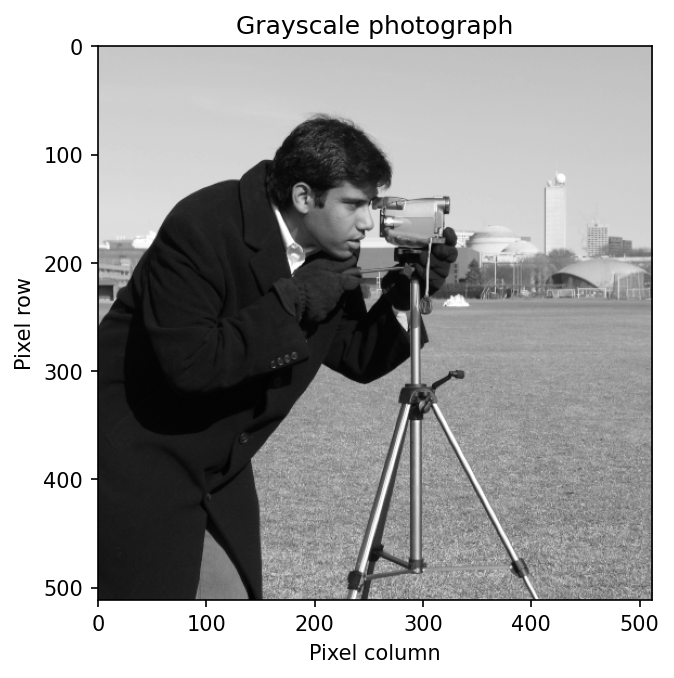
\includegraphics[width=.46\linewidth]{grayscale_image.png}\hfill
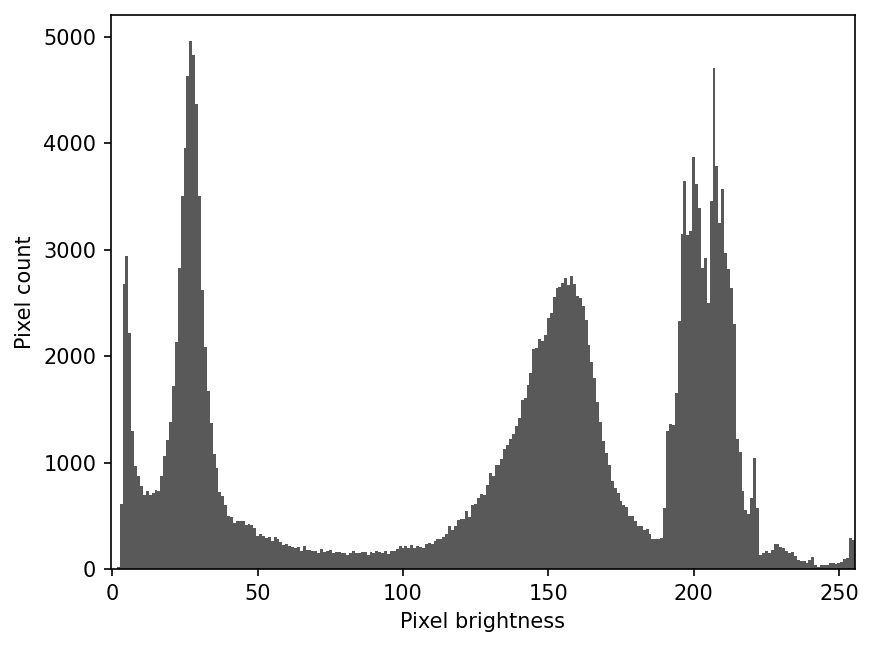
\includegraphics[width=.51\linewidth]{brightness_histogram.png}
\end{center}
{\small\textbf{Figure 1.} The dark silhouette and coat contribute to the low-brightness peak. The lighter background occupies a different part of the histogram. A histogram counts intensities and discards their positions.}\par
The Python loader recovered 262,144 unsigned 8-bit samples, with zero missing entries. Measured brightness ranged from 0 to 255 with mean 129.06. The PNG decoder returns normalized samples, which the loader multiplies by 255 and rounds to integer levels. The algebra below uses real-valued arithmetic.\par
{\small Photograph: Lav Varshney, CC0, via \href{https://scikit-image.org/docs/0.25.x/api/skimage.data.html#skimage.data.camera}{scikit-image's camera dataset}.}
\newpage
\head{Notation, definitions and assumptions}
\begin{tabularx}{\linewidth}{@{}l l X@{}}\toprule
Symbol & Dimensions & Meaning\\\midrule
$m,n$; $i,j$ & integers & Image height and width; indices with bounds set by the sum or matrix.\\
$A,A_k$ & $m\times n$ & Real data matrix and its approximation retaining $k$ components.\\
$r,k$ & integers & $r=\operatorname{rank}(A)$; $0\leq k\leq r$.\\
$G,V,\Lambda$ & $n\times n$ & Gram matrix, full orthogonal eigenbasis, diagonal eigenvalue matrix.\\
$\lambda_i,\sigma_i$ & scalars & Ordered Gram eigenvalues and their nonnegative square roots.\\
$v_i,u_i$ & $n\times1$, $m\times1$ & Right singular vector and its left partner when $\sigma_i>0$.\\
$V_k,U_k,\Sigma_k$ & $n\times k$, $m\times k$, $k\times k$ & First $k$ vectors and diagonal matrix of their singular values.\\
$I_d,\delta_{ij}$ & $d\times d$, scalar & Identity and Kronecker delta ($1$ for $i=j$, $0$ otherwise).\\
$x,M,N$ & $n\times1$, conformable & Test vector and generic matrices. Superscript $\top$ denotes transpose.\\
$L,R$ & $120\times5$, $5\times80$ & Random left and right factors in the simulation.\\
$Z,B$ & $120\times80$ each & Standard-normal noise and the clean signal $B=LR$.\\
\bottomrule\end{tabularx}
\subhead{Definitions}
Rank is the dimension of the column space, the span of the matrix's columns. A Gram matrix $G=A^\top A$ contains their pairwise inner products. A real symmetric matrix is positive semidefinite (PSD) if $x^\top Gx\geq0$ for every $x$. An eigenpair satisfies $Gv_i=\lambda_i v_i$ with $v_i\ne0$. Orthonormal vectors satisfy $v_i^\top v_j=\delta_{ij}$. An outer product $u_iv_i^\top$ maps $x$ to $u_i(v_i^\top x)$.
The compact SVD is $A=U_r\Sigma_rV_r^\top$ with orthonormal columns in both factors and positive diagonal entries in descending order. Truncation keeps the first $k$ terms. The trace is the sum of diagonal entries. The Frobenius inner product is $\langle M,N\rangle_F=\tr(M^\top N)$, and $\|M\|_F^2=\sum_{ij}M_{ij}^2$.
\subhead{Conditions and Iteration 3 checks}
\small
\begin{tabularx}{\linewidth}{@{}p{.24\linewidth} X X@{}}\toprule
Condition & Consequence if violated & Check on the photograph\\\midrule
Complete finite grayscale grid & Undefined entries invalidate the ordinary Gram product; a color tuple is not a scalar. & Check shape, channels, finite count, type and brightness range before converting to float.\\
Orthonormal eigenbasis; positive retained values & Cross terms can survive; division by zero cannot define $u_i$. & Order eigenvalues, apply a roundoff tolerance, check both factor Gram matrices.\\
Unweighted squared pixel error & The discarded tail predicts this loss. Perceptual scores and rounded outputs can differ. & Check the identity before display rounding; inspect edges visually as a separate evaluation.\\
Comparable scalar storage & Unequal element widths or encoded files change the byte comparison. & Count factor entries and record their dtype and actual file sizes separately.\\\bottomrule
\end{tabularx}\normalsize
\newpage
\head{Iteration 2 -- Math Questions}
\subhead{Q1. The Gram matrix has a nonnegative spectrum}
\review{Jiaxiao Chen}{Alexander Rees}
\textbf{Proposition.} $A^\top A$ is symmetric and PSD. Its eigenvalues are real and nonnegative, so $\sigma_i=\sqrt{\lambda_i}$ is well-defined.
\begin{align*}
G^\top&=(A^\top A)^\top=A^\top(A^\top)^\top=A^\top A
&&\text{(transpose of a product and involution)},\\
x^\top Gx&=x^\top A^\top Ax=(Ax)^\top(Ax)=\|Ax\|_2^2\geq0
&&\text{(associativity and squared length)}.
\end{align*}
The real spectral theorem supplies an orthonormal eigenbasis of $G$ and real eigenvalues. For each unit eigenvector, $0\leq v_i^\top Gv_i=\lambda_i v_i^\top v_i=\lambda_i$ by the eigenvector equation and normalization. Order the eigenvalues decreasingly and take their nonnegative square roots. \proofend
\subhead{Q2. Constructing orthonormal left singular vectors}
\review{Jiaxiao Chen}{Alexander Rees}
\textbf{Proposition.} For $\sigma_i>0$, letting $u_i=Av_i/\sigma_i$ gives $Av_i=\sigma_i u_i$ and $u_i^\top u_j=\delta_{ij}$.
First, $\|Av_i\|_2^2=v_i^\top Gv_i=\lambda_i$ by Q1. Taking the square root gives $\|Av_i\|_2=\sigma_i$, so normalization gives the stated $u_i$. For two positive singular values,
\[
u_i^\top u_j
=\frac{v_i^\top A^\top A v_j}{\sigma_i\sigma_j}
=\frac{\lambda_j v_i^\top v_j}{\sigma_i\sigma_j}
=\frac{\lambda_j\delta_{ij}}{\sigma_i\sigma_j}.
\]
The equalities use the transpose rule, the eigenvector equation, and orthonormality of the chosen basis. For $i\ne j$ the result is zero. For $i=j$ it is $\lambda_i/\sigma_i^2=1$. In a repeated eigenspace the spectral theorem still permits an orthonormal basis. If $\lambda_i=0$, then $\|Av_i\|_2=0$ and $Av_i=0$. \proofend
\subhead{Q3. The rank-one expansion}
\review{Jiaxiao Chen}{Alexander Rees}
\textbf{Proposition.} $A=\sum_{i=1}^r \sigma_i u_i v_i^\top$.
Since the columns of $V$ form a complete orthonormal basis, $VV^\top=I_n$. Expanding this product column by column and distributing $A$ gives
\[
A=AI_n=A\sum_{i=1}^n v_iv_i^\top
=\sum_{i=1}^n(Av_i)v_i^\top
=\sum_{i=1}^r \sigma_i u_i v_i^\top.
\]
For the last step, Q2 replaces each positive term and eliminates the zero terms. Indeed, $Gx=0$ implies $\|Ax\|_2^2=x^\top Gx=0$; conversely $Ax=0$ implies $Gx=0$. Rank--nullity therefore gives $\operatorname{rank}(G)=r$, the number of positive eigenvalues. Each remaining outer product has image $\operatorname{span}(u_i)$ since it maps $v_i$ to $u_i$ and every other vector into that line. \proofend
\newpage
\head{Energy and the price of truncation}
\subhead{Q4. Frobenius energy is the sum of squared singular values}
\review{Alexander Rees}{Jiaxiao Chen}
\textbf{Proposition.} $\|A\|_F^2=\tr(A^\top A)=\sum_{i=1}^r\sigma_i^2$.
The $j$th diagonal entry of $A^\top A$ is the dot product of column $j$ with itself. Therefore
\[
\tr(A^\top A)
=\sum_{j=1}^{n}(A^\top A)_{jj}
=\sum_{j=1}^{n}\sum_{i=1}^{m}A_{ij}^2
=\|A\|_F^2
\]
by the trace definition, matrix multiplication and the Frobenius norm definition. From $G=V\Lambda V^\top$, cyclic invariance of trace gives
\[
\tr(G)=\tr(\Lambda V^\top V)=\tr(\Lambda)=\sum_{i=1}^n\lambda_i
=\sum_{i=1}^r\sigma_i^2.
\]
Here $V^\top V=I_n$ by orthogonality, and exactly $r$ eigenvalues are positive by Q3. \proofend
\subhead{Q5. Error and storage at rank \texorpdfstring{$k$}{k}}
\review{Alexander Rees}{Jiaxiao Chen}
\textbf{Proposition.} For $A_k=\sum_{i=1}^k\sigma_i u_iv_i^\top$,
\[
\|A-A_k\|_F^2=\sum_{i=k+1}^r\sigma_i^2,\qquad
\text{factor storage}=k(m+n+1)\ \text{scalars}.
\]
Subtract the first $k$ summands from Q3. To measure the squared norm of the remaining sum, write $M_i=u_iv_i^\top$. The trace identity for the Frobenius inner product gives
\begin{align*}
\langle M_i,M_j\rangle_F
&=\tr(v_i u_i^\top u_j v_j^\top) &&\text{(transpose of an outer product)}\\
&=(u_i^\top u_j)\tr(v_iv_j^\top) &&\text{(linearity in scalar factors)}\\
&=(u_i^\top u_j)(v_j^\top v_i)=\delta_{ij} &&\text{(trace and orthonormality).}
\end{align*}
Bilinearity now yields $\|A-A_k\|_F^2=\sum_{i,j>k}\sigma_i\sigma_j\delta_{ij}
=\sum_{i>k}\sigma_i^2$. This also gives the full energy at $k=0$ and zero error at $k=r$.
Each component needs $m$ entries of $u_i$, $n$ entries of $v_i$ and one weight. Adding their counts gives $mk+nk+k=k(m+n+1)$. \proofend
\subhead{Interpreting the storage threshold}
At equal precision the factors save entries exactly when $k<mn/(m+n+1)$. On the $512\times512$ photograph that permits $k\leq255$. If pixels use one byte and each factor entry uses eight, the corresponding raw-byte inequality is $8k(1025)<262144$, allowing only $k\leq31$. Both comparisons exclude headers and PNG coding.
\newpage
\head{Algorithm and simulation design}
\subhead{Computing a rank-\texorpdfstring{$k$}{k} approximation}
The following dense algorithm assumes real arithmetic. The operation counts use conventional matrix multiplication; $O(\cdot)$ bounds arithmetic growth as the dimensions increase.
\begin{enumerate}
\item \textbf{Read the image.} Convert each brightness value to floating point to form $A\in\mathbb R^{m\times n}$. Reading and converting all entries costs $O(mn)$.
\item \textbf{Build the Gram matrix.} Set $G=A^\top A\in\mathbb R^{n\times n}$. Computing all entries directly takes $mn^2$ multiplications and $(m-1)n^2$ additions.
\item \textbf{Find eigenpairs.} Diagonalize the real symmetric $G=V\Lambda V^\top$ with a dense symmetric eigensolver, $O(n^3)$. The implementation reverses the ascending eigenpairs. Copying all columns in reverse order costs at most $O(n^2)$.
\item \textbf{Select components.} Set $\sigma_i=\sqrt{\max(\lambda_i,0)}$ for $n$ eigenvalues, $O(n)$. For numerical division, retain eigenvalues above $\tau=\epsilon\max(m,n)\lambda_1$, where $\epsilon$ is machine precision. Check the smallest eigenvalue against $-\tau$. Choose $k$ within the count of retained values.
\item \textbf{Encode.} Form $U_k=(AV_k)\Sigma_k^{-1}$ by dividing each of $k$ columns by its own weight. Shapes are $m\times k$, $n\times k$ and $k\times k$ for $U_k,V_k,\Sigma_k$. The product takes $mnk$ multiplications and $mk(n-1)$ additions, followed by $mk$ divisions. Store the diagonal as a length-$k$ vector.
\item \textbf{Decode and check.} Scale the columns of $U_k$ by their weights ($mk$ multiplications) and multiply by $V_k^\top$ to recover $A_k\in\mathbb R^{m\times n}$ ($mnk$ multiplications and $mn(k-1)$ additions for $k\geq1$). For $k=0$, return the zero matrix. Evaluating the squared pixel error costs $O(mn)$, and summing the discarded eigenvalues costs $O(n-k)$.
\end{enumerate}
The simulation forms every positive left singular vector once so that several ranks can reuse the same decomposition. Forming $A^\top A$ squares the ratio of the largest to smallest positive singular values. Very small components can consequently be hard to recover. NumPy's direct SVD supplies the final independent numerical comparison.
\subhead{Simulation Check}
With seed zero and NumPy's default random generator, draw $L\in\mathbb R^{120\times5}$, $R\in\mathbb R^{5\times80}$, and then $Z\in\mathbb R^{120\times80}$ with independent standard-normal entries. Define the clean signal $B=LR$ and observed matrix $A=B+0.01Z$. This gives one synthetic image with 9,600 entries. Its real-valued intensities are left unclipped, since rounding would change the algebraic test.\par
The clean factors have full rank five with probability one, and the script verifies five eigenvalues above tolerance on this draw. The clean singular values below are square roots of the five largest eigenvalues of $B^\top B$. All remaining clean singular values are zero.
\newpage
\head{Simulation Check \textnormal{\large / results}}
\begin{center}
\begin{tabular}{@{}rrrrrrr@{}}\toprule
Component $i$ & 1 & 2 & 3 & 4 & 5 & 6\\\midrule
Clean truth &109.1427&100.3853&94.8936&78.4417&71.8757&0.0000\\
Noisy estimate &109.1511&100.3751&94.8887&78.4231&71.8822&0.1899\\\bottomrule
\end{tabular}
\end{center}
The fifth observed singular value is 378.51 times the sixth. The gap identifies the five dominant signal directions even though the noise gives the observed matrix 80 positive singular values.
\begin{center}
\begin{tabular}{@{}rrrrr@{}}\toprule
$k$ & Measured $\|A-A_k\|_F^2$ & Predicted $\sum_{i>k}\sigma_i^2$ & Stored scalars & Share of 9,600\\\midrule
1 &30397.117615&30397.117615&201&2.09\%\\
3 &11318.104147&11318.104147&603&6.28\%\\
5 &0.873022&0.873022&1005&10.47\%\\
10&0.707677&0.707677&2010&20.94\%\\\bottomrule
\end{tabular}
\end{center}
\textbf{Q1.} The noisy Gram matrix passed the symmetry check and its smallest eigenvalue was $4.89617\times10^{-4}$, consistent with positive semidefiniteness.\par
\textbf{Q2.} The largest absolute entry of $U^\top U-I_{80}$ was $6.62\times10^{-10}$, consistent with orthonormal recovered columns.\par
\textbf{Q3.} Summing all rank-one components recovered the noisy input to a maximum absolute entrywise difference of $1.51\times10^{-14}$.\par
\textbf{Q4.} The direct sum of squared entries, Gram trace, and sum of squared singular values each gave $42311.07686990$ to the precision shown.\par
\textbf{Q5.} At every listed rank the measured squared residual agreed with the tail prediction. Rank five kept $99.9979\%$ of the observed energy using 1,005 scalars. Doubling factor storage to rank ten reduced the remaining squared error by only $0.165345$.\par
The final direct-SVD comparison gave a maximum absolute singular-value difference of $6.10\times10^{-12}$. Last digits can vary with the numerical library.
\subhead{Team review record}\label{review}
Owners and assigned checkers are listed above each proof. Each person should sign below after completing their own review.
\begin{center}
\begin{tabularx}{\linewidth}{@{}lXX@{}}\toprule
Questions & Owner signature & Checked by (signature)\\\midrule
Q1--Q3 & Jiaxiao Chen: \hrulefill & Alexander Rees: \hrulefill\\[5pt]
Q4--Q5 & Alexander Rees: \hrulefill & Jiaxiao Chen: \hrulefill\\\bottomrule
\end{tabularx}
\end{center}
{\small\textbf{Reproducibility.} Run \texttt{src/load\_image.py} and \texttt{src/simulate\_svd.py} in the \href{https://github.com/Alexander-Rees/DS5020-SVD-Image-Compression}{team repository}. See its README for the image and commands.}
\end{document}
